\documentclass{standalone}
\usepackage{tikz}
\usetikzlibrary{patterns, positioning}


\begin{document}
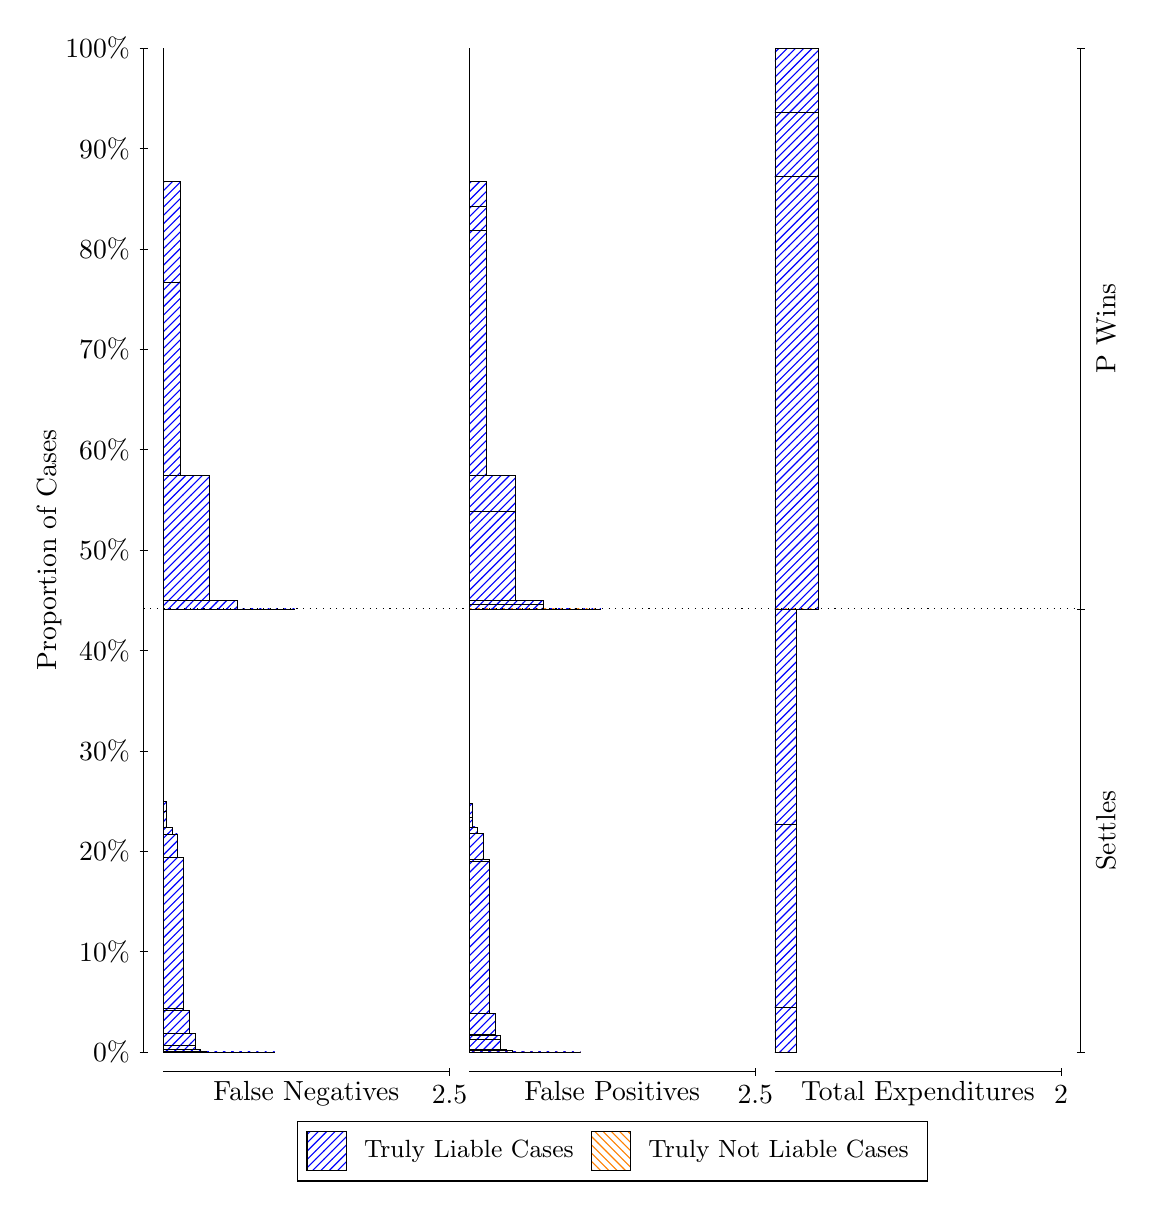
\begin{tikzpicture}
\draw[black, very thin] (1.5,1.75) -- (1.5,14.5);
\node[rotate=90, text=black, anchor=center] at (0.3, 8.125) {Proportion of Cases};
\draw[black, very thin] (1.45,1.75) -- (1.55,1.75);
\node[text=black, anchor=east] at (1.45, 1.75) {0\%};
\draw[black, very thin] (1.45,3.025) -- (1.55,3.025);
\node[text=black, anchor=east] at (1.45, 3.025) {10\%};
\draw[black, very thin] (1.45,4.3) -- (1.55,4.3);
\node[text=black, anchor=east] at (1.45, 4.3) {20\%};
\draw[black, very thin] (1.45,5.575) -- (1.55,5.575);
\node[text=black, anchor=east] at (1.45, 5.575) {30\%};
\draw[black, very thin] (1.45,6.85) -- (1.55,6.85);
\node[text=black, anchor=east] at (1.45, 6.85) {40\%};
\draw[black, very thin] (1.45,8.125) -- (1.55,8.125);
\node[text=black, anchor=east] at (1.45, 8.125) {50\%};
\draw[black, very thin] (1.45,9.4) -- (1.55,9.4);
\node[text=black, anchor=east] at (1.45, 9.4) {60\%};
\draw[black, very thin] (1.45,10.675) -- (1.55,10.675);
\node[text=black, anchor=east] at (1.45, 10.675) {70\%};
\draw[black, very thin] (1.45,11.95) -- (1.55,11.95);
\node[text=black, anchor=east] at (1.45, 11.95) {80\%};
\draw[black, very thin] (1.45,13.225) -- (1.55,13.225);
\node[text=black, anchor=east] at (1.45, 13.225) {90\%};
\draw[black, very thin] (1.45,14.5) -- (1.55,14.5);
\node[text=black, anchor=east] at (1.45, 14.5) {100\%};

\draw[black, very thin] (13.4,1.75) -- (13.4,14.5);
\draw[black, very thin] (13.35,1.75) -- (13.45,1.75);
\node[anchor=west] at (13.35, 1.75) {};
\draw[black, very thin] (13.35,7.3773) -- (13.45,7.3773);
\node[anchor=west] at (13.35, 7.3773) {};
\draw[black, very thin] (13.35,14.5) -- (13.45,14.5);
\node[anchor=west] at (13.35, 14.5) {};

\draw[black, very thin, pattern color=blue, pattern=north east lines] (1.75,1.75) rectangle (3.167,1.75);
\draw[black, very thin, pattern color=blue, pattern=north east lines] (1.75,1.75) rectangle (3.0217,1.75);
\draw[black, very thin, pattern color=blue, pattern=north east lines] (1.75,1.75) rectangle (2.8763,1.75);
\draw[black, very thin, pattern color=blue, pattern=north east lines] (1.75,1.75) rectangle (2.8037,1.75);
\draw[black, very thin, pattern color=blue, pattern=north east lines] (1.75,1.75) rectangle (2.731,1.75);
\draw[black, very thin, pattern color=blue, pattern=north east lines] (1.75,1.75) rectangle (2.6583,1.75);
\draw[black, very thin, pattern color=blue, pattern=north east lines] (1.75,1.75) rectangle (2.5857,1.75);
\draw[black, very thin, pattern color=blue, pattern=north east lines] (1.75,1.75) rectangle (2.513,1.7503);
\draw[black, very thin, pattern color=blue, pattern=north east lines] (1.75,1.7503) rectangle (2.4403,1.7519);
\draw[black, very thin, pattern color=blue, pattern=north east lines] (1.75,1.7519) rectangle (2.3677,1.7519);
\draw[black, very thin, pattern color=blue, pattern=north east lines] (1.75,1.7519) rectangle (2.3677,1.7522);
\draw[black, very thin, pattern color=blue, pattern=north east lines] (1.75,1.7522) rectangle (2.295,1.7644);
\draw[black, very thin, pattern color=blue, pattern=north east lines] (1.75,1.7644) rectangle (2.2223,1.7844);
\draw[black, very thin, pattern color=blue, pattern=north east lines] (1.75,1.7844) rectangle (2.1497,1.8371);
\draw[black, very thin, pattern color=blue, pattern=north east lines] (1.75,1.8371) rectangle (2.1497,1.9847);
\draw[black, very thin, pattern color=blue, pattern=north east lines] (1.75,1.9847) rectangle (2.077,2.2741);
\draw[black, very thin, pattern color=blue, pattern=north east lines] (1.75,2.2741) rectangle (2.0043,2.2742);
\draw[black, very thin, pattern color=blue, pattern=north east lines] (1.75,2.2742) rectangle (2.0043,2.2996);
\draw[black, very thin, pattern color=blue, pattern=north east lines] (1.75,2.2996) rectangle (2.0043,4.2204);
\draw[black, very thin, pattern color=blue, pattern=north east lines] (1.75,4.2204) rectangle (1.9317,4.5184);
\draw[black, very thin, pattern color=blue, pattern=north east lines] (1.75,4.5184) rectangle (1.859,4.6002);
\draw[black, very thin, pattern color=blue, pattern=north east lines] (1.75,4.6002) rectangle (1.7863,4.8051);
\draw[black, very thin, pattern color=blue, pattern=north east lines] (1.75,4.8051) rectangle (1.7863,4.9321);
\draw[black, very thin, pattern color=orange, pattern=north west lines] (1.75,4.9321) rectangle (1.75,4.9321);
\draw[black, very thin, pattern color=blue, pattern=north east lines] (1.75,4.9321) rectangle (1.75,7.3773);
\draw[black, very thin, pattern color=blue, pattern=north east lines] (1.75,7.3773) rectangle (3.4213,7.3773);
\draw[black, very thin, pattern color=blue, pattern=north east lines] (1.75,7.3773) rectangle (3.058,7.3785);
\draw[black, very thin, pattern color=blue, pattern=north east lines] (1.75,7.3785) rectangle (2.6947,7.4887);
\draw[black, very thin, pattern color=blue, pattern=north east lines] (1.75,7.4887) rectangle (2.3313,9.075);
\draw[black, very thin, pattern color=blue, pattern=north east lines] (1.75,9.075) rectangle (1.968,11.521);
\draw[black, very thin, pattern color=blue, pattern=north east lines] (1.75,11.521) rectangle (1.968,12.803);
\draw[black, very thin, pattern color=orange, pattern=north west lines] (1.75,12.803) rectangle (1.75,12.803);
\draw[black, very thin, pattern color=blue, pattern=north east lines] (1.75,12.803) rectangle (1.75,14.5);
\draw[black, very thin, pattern color=orange, pattern=north west lines] (5.6333,1.75) rectangle (7.0503,1.75);
\draw[black, very thin, pattern color=blue, pattern=north east lines] (5.6333,1.75) rectangle (7.0503,1.75);
\draw[black, very thin, pattern color=orange, pattern=north west lines] (5.6333,1.75) rectangle (6.905,1.75);
\draw[black, very thin, pattern color=blue, pattern=north east lines] (5.6333,1.75) rectangle (6.905,1.75);
\draw[black, very thin, pattern color=orange, pattern=north west lines] (5.6333,1.75) rectangle (6.7597,1.75);
\draw[black, very thin, pattern color=blue, pattern=north east lines] (5.6333,1.75) rectangle (6.7597,1.75);
\draw[black, very thin, pattern color=blue, pattern=north east lines] (5.6333,1.75) rectangle (6.687,1.75);
\draw[black, very thin, pattern color=orange, pattern=north west lines] (5.6333,1.75) rectangle (6.6143,1.75);
\draw[black, very thin, pattern color=blue, pattern=north east lines] (5.6333,1.75) rectangle (6.6143,1.75);
\draw[black, very thin, pattern color=blue, pattern=north east lines] (5.6333,1.75) rectangle (6.5417,1.75);
\draw[black, very thin, pattern color=orange, pattern=north west lines] (5.6333,1.75) rectangle (6.469,1.75);
\draw[black, very thin, pattern color=blue, pattern=north east lines] (5.6333,1.75) rectangle (6.469,1.75);
\draw[black, very thin, pattern color=blue, pattern=north east lines] (5.6333,1.75) rectangle (6.3963,1.7502);
\draw[black, very thin, pattern color=orange, pattern=north west lines] (5.6333,1.7502) rectangle (6.3237,1.7502);
\draw[black, very thin, pattern color=blue, pattern=north east lines] (5.6333,1.7502) rectangle (6.3237,1.7503);
\draw[black, very thin, pattern color=orange, pattern=north west lines] (5.6333,1.7503) rectangle (6.3237,1.7503);
\draw[black, very thin, pattern color=blue, pattern=north east lines] (5.6333,1.7503) rectangle (6.3237,1.7517);
\draw[black, very thin, pattern color=blue, pattern=north east lines] (5.6333,1.7517) rectangle (6.251,1.752);
\draw[black, very thin, pattern color=orange, pattern=north west lines] (5.6333,1.752) rectangle (6.1783,1.752);
\draw[black, very thin, pattern color=blue, pattern=north east lines] (5.6333,1.752) rectangle (6.1783,1.7654);
\draw[black, very thin, pattern color=blue, pattern=north east lines] (5.6333,1.7654) rectangle (6.1057,1.783);
\draw[black, very thin, pattern color=orange, pattern=north west lines] (5.6333,1.783) rectangle (6.033,1.783);
\draw[black, very thin, pattern color=blue, pattern=north east lines] (5.6333,1.783) rectangle (6.033,1.9158);
\draw[black, very thin, pattern color=blue, pattern=north east lines] (5.6333,1.9158) rectangle (6.033,1.9572);
\draw[black, very thin, pattern color=blue, pattern=north east lines] (5.6333,1.9572) rectangle (5.9603,1.9742);
\draw[black, very thin, pattern color=blue, pattern=north east lines] (5.6333,1.9742) rectangle (5.9603,2.2375);
\draw[black, very thin, pattern color=orange, pattern=north west lines] (5.6333,2.2375) rectangle (5.8877,2.2375);
\draw[black, very thin, pattern color=blue, pattern=north east lines] (5.6333,2.2375) rectangle (5.8877,4.1733);
\draw[black, very thin, pattern color=blue, pattern=north east lines] (5.6333,4.1733) rectangle (5.8877,4.1953);
\draw[black, very thin, pattern color=blue, pattern=north east lines] (5.6333,4.1953) rectangle (5.815,4.5272);
\draw[black, very thin, pattern color=blue, pattern=north east lines] (5.6333,4.5272) rectangle (5.7423,4.6089);
\draw[black, very thin, pattern color=blue, pattern=north east lines] (5.6333,4.6089) rectangle (5.6697,4.7263);
\draw[black, very thin, pattern color=blue, pattern=north east lines] (5.6333,4.7263) rectangle (5.6697,4.9069);
\draw[black, very thin, pattern color=blue, pattern=north east lines] (5.6333,4.9069) rectangle (5.6333,7.3773);
\draw[black, very thin, pattern color=orange, pattern=north west lines] (5.6333,7.3773) rectangle (7.3047,7.3773);
\draw[black, very thin, pattern color=blue, pattern=north east lines] (5.6333,7.3773) rectangle (7.3047,7.3773);
\draw[black, very thin, pattern color=orange, pattern=north west lines] (5.6333,7.3773) rectangle (6.9413,7.3773);
\draw[black, very thin, pattern color=blue, pattern=north east lines] (5.6333,7.3773) rectangle (6.9413,7.3776);
\draw[black, very thin, pattern color=blue, pattern=north east lines] (5.6333,7.3776) rectangle (6.9413,7.3784);
\draw[black, very thin, pattern color=orange, pattern=north west lines] (5.6333,7.3784) rectangle (6.578,7.3784);
\draw[black, very thin, pattern color=blue, pattern=north east lines] (5.6333,7.3784) rectangle (6.578,7.4363);
\draw[black, very thin, pattern color=blue, pattern=north east lines] (5.6333,7.4363) rectangle (6.578,7.4881);
\draw[black, very thin, pattern color=orange, pattern=north west lines] (5.6333,7.4881) rectangle (6.2147,7.4881);
\draw[black, very thin, pattern color=blue, pattern=north east lines] (5.6333,7.4881) rectangle (6.2147,8.6171);
\draw[black, very thin, pattern color=blue, pattern=north east lines] (5.6333,8.6171) rectangle (6.2147,9.074);
\draw[black, very thin, pattern color=blue, pattern=north east lines] (5.6333,9.074) rectangle (5.8513,12.18);
\draw[black, very thin, pattern color=orange, pattern=north west lines] (5.6333,12.18) rectangle (5.8513,12.18);
\draw[black, very thin, pattern color=blue, pattern=north east lines] (5.6333,12.18) rectangle (5.8513,12.491);
\draw[black, very thin, pattern color=blue, pattern=north east lines] (5.6333,12.491) rectangle (5.8513,12.802);
\draw[black, very thin, pattern color=blue, pattern=north east lines] (5.6333,12.802) rectangle (5.6333,14.5);
\draw[black, very thin, pattern color=orange, pattern=north west lines] (9.5167,1.75) rectangle (9.7892,1.75);
\draw[black, very thin, pattern color=blue, pattern=north east lines] (9.5167,1.75) rectangle (9.7892,2.3145);
\draw[black, very thin, pattern color=orange, pattern=north west lines] (9.5167,2.3145) rectangle (9.7892,2.3145);
\draw[black, very thin, pattern color=blue, pattern=north east lines] (9.5167,2.3145) rectangle (9.7892,4.6452);
\draw[black, very thin, pattern color=orange, pattern=north west lines] (9.5167,4.6452) rectangle (9.7892,4.6452);
\draw[black, very thin, pattern color=blue, pattern=north east lines] (9.5167,4.6452) rectangle (9.7892,7.3773);
\draw[black, very thin, pattern color=orange, pattern=north west lines] (9.5167,7.3773) rectangle (10.062,7.3773);
\draw[black, very thin, pattern color=blue, pattern=north east lines] (9.5167,7.3773) rectangle (10.062,12.865);
\draw[black, very thin, pattern color=orange, pattern=north west lines] (9.5167,12.865) rectangle (10.062,12.865);
\draw[black, very thin, pattern color=blue, pattern=north east lines] (9.5167,12.865) rectangle (10.062,13.679);
\draw[black, very thin, pattern color=orange, pattern=north west lines] (9.5167,13.679) rectangle (10.062,13.679);
\draw[black, very thin, pattern color=blue, pattern=north east lines] (9.5167,13.679) rectangle (10.062,14.5);
\draw[black, dotted] (1.5,7.3773) -- (13.4,7.3773);
\draw[black, very thin] (1.75,1.5) -- (5.3833,1.5);
\node[text=black, anchor=north] at (3.5667, 1.5) {False Negatives};
\draw[black, very thin] (5.3833,1.45) -- (5.3833,1.55);
\node[text=black, anchor=north] at (5.3833, 1.45) {2.5};

\draw[black, very thin] (5.6333,1.5) -- (9.2667,1.5);
\node[text=black, anchor=north] at (7.45, 1.5) {False Positives};
\draw[black, very thin] (9.2667,1.45) -- (9.2667,1.55);
\node[text=black, anchor=north] at (9.2667, 1.45) {2.5};

\draw[black, very thin] (9.5167,1.5) -- (13.15,1.5);
\node[text=black, anchor=north] at (11.333, 1.5) {Total Expenditures};
\draw[black, very thin] (13.15,1.45) -- (13.15,1.55);
\node[text=black, anchor=north] at (13.15, 1.45) {2};

\node[text=black, centered, rotate=90] at (13.72, 4.5637) {Settles};
\node[text=black, centered, rotate=90] at (13.72, 10.939) {P Wins};

\draw (7.449999999999999,1.5) node[draw=none] (baseCoordinate) {};
\begin{scope}[align=center]
        \matrix[scale=0.5, draw=black, below=0.5cm of baseCoordinate, nodes={draw}, column sep=0.1cm]{
            \node[rectangle, draw, minimum width=0.5cm, minimum height=0.5cm, pattern color=blue, pattern=north east lines] {}; &
            \node[draw=none, font=\small, text=black] (B) {Truly Liable Cases}; &
            \node[rectangle, draw, minimum width=0.5cm, minimum height=0.5cm, pattern color=orange, pattern=north west lines] {}; &
            \node[draw=none, font=\small, text=black] (B) {Truly Not Liable Cases}; \\
            };
\end{scope}

\end{tikzpicture}
\end{document}